\begin{frame}
  \frametitle{Control Rods in MSRs}
  \begin{columns}
    \hfill
    \column[t]{5cm}
    \begin{figure}
      \centering
      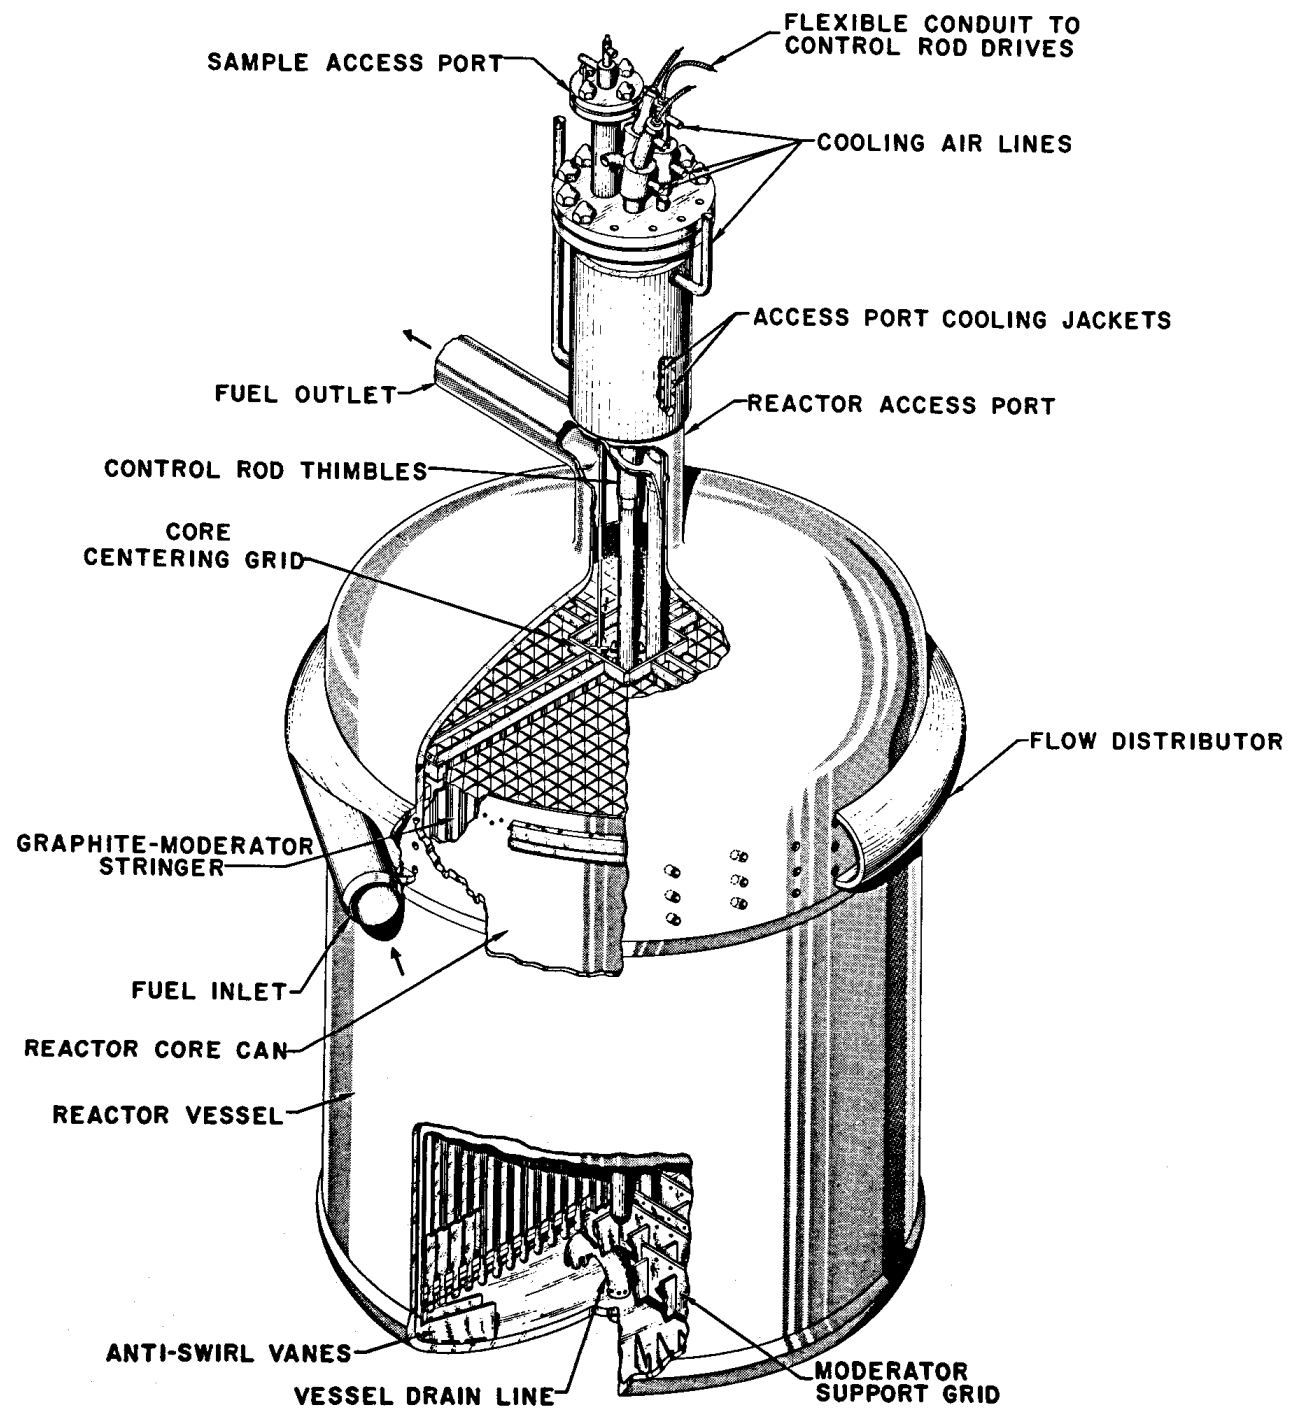
\includegraphics[width=\columnwidth]{images/msre-cutout}
      \caption{\footnotesize MSRE reactor vessel \cite{robertson_msre_1965}}
    \end{figure}
    \hfill
    \column[t]{6cm}
    \begin{figure}
      \centering
      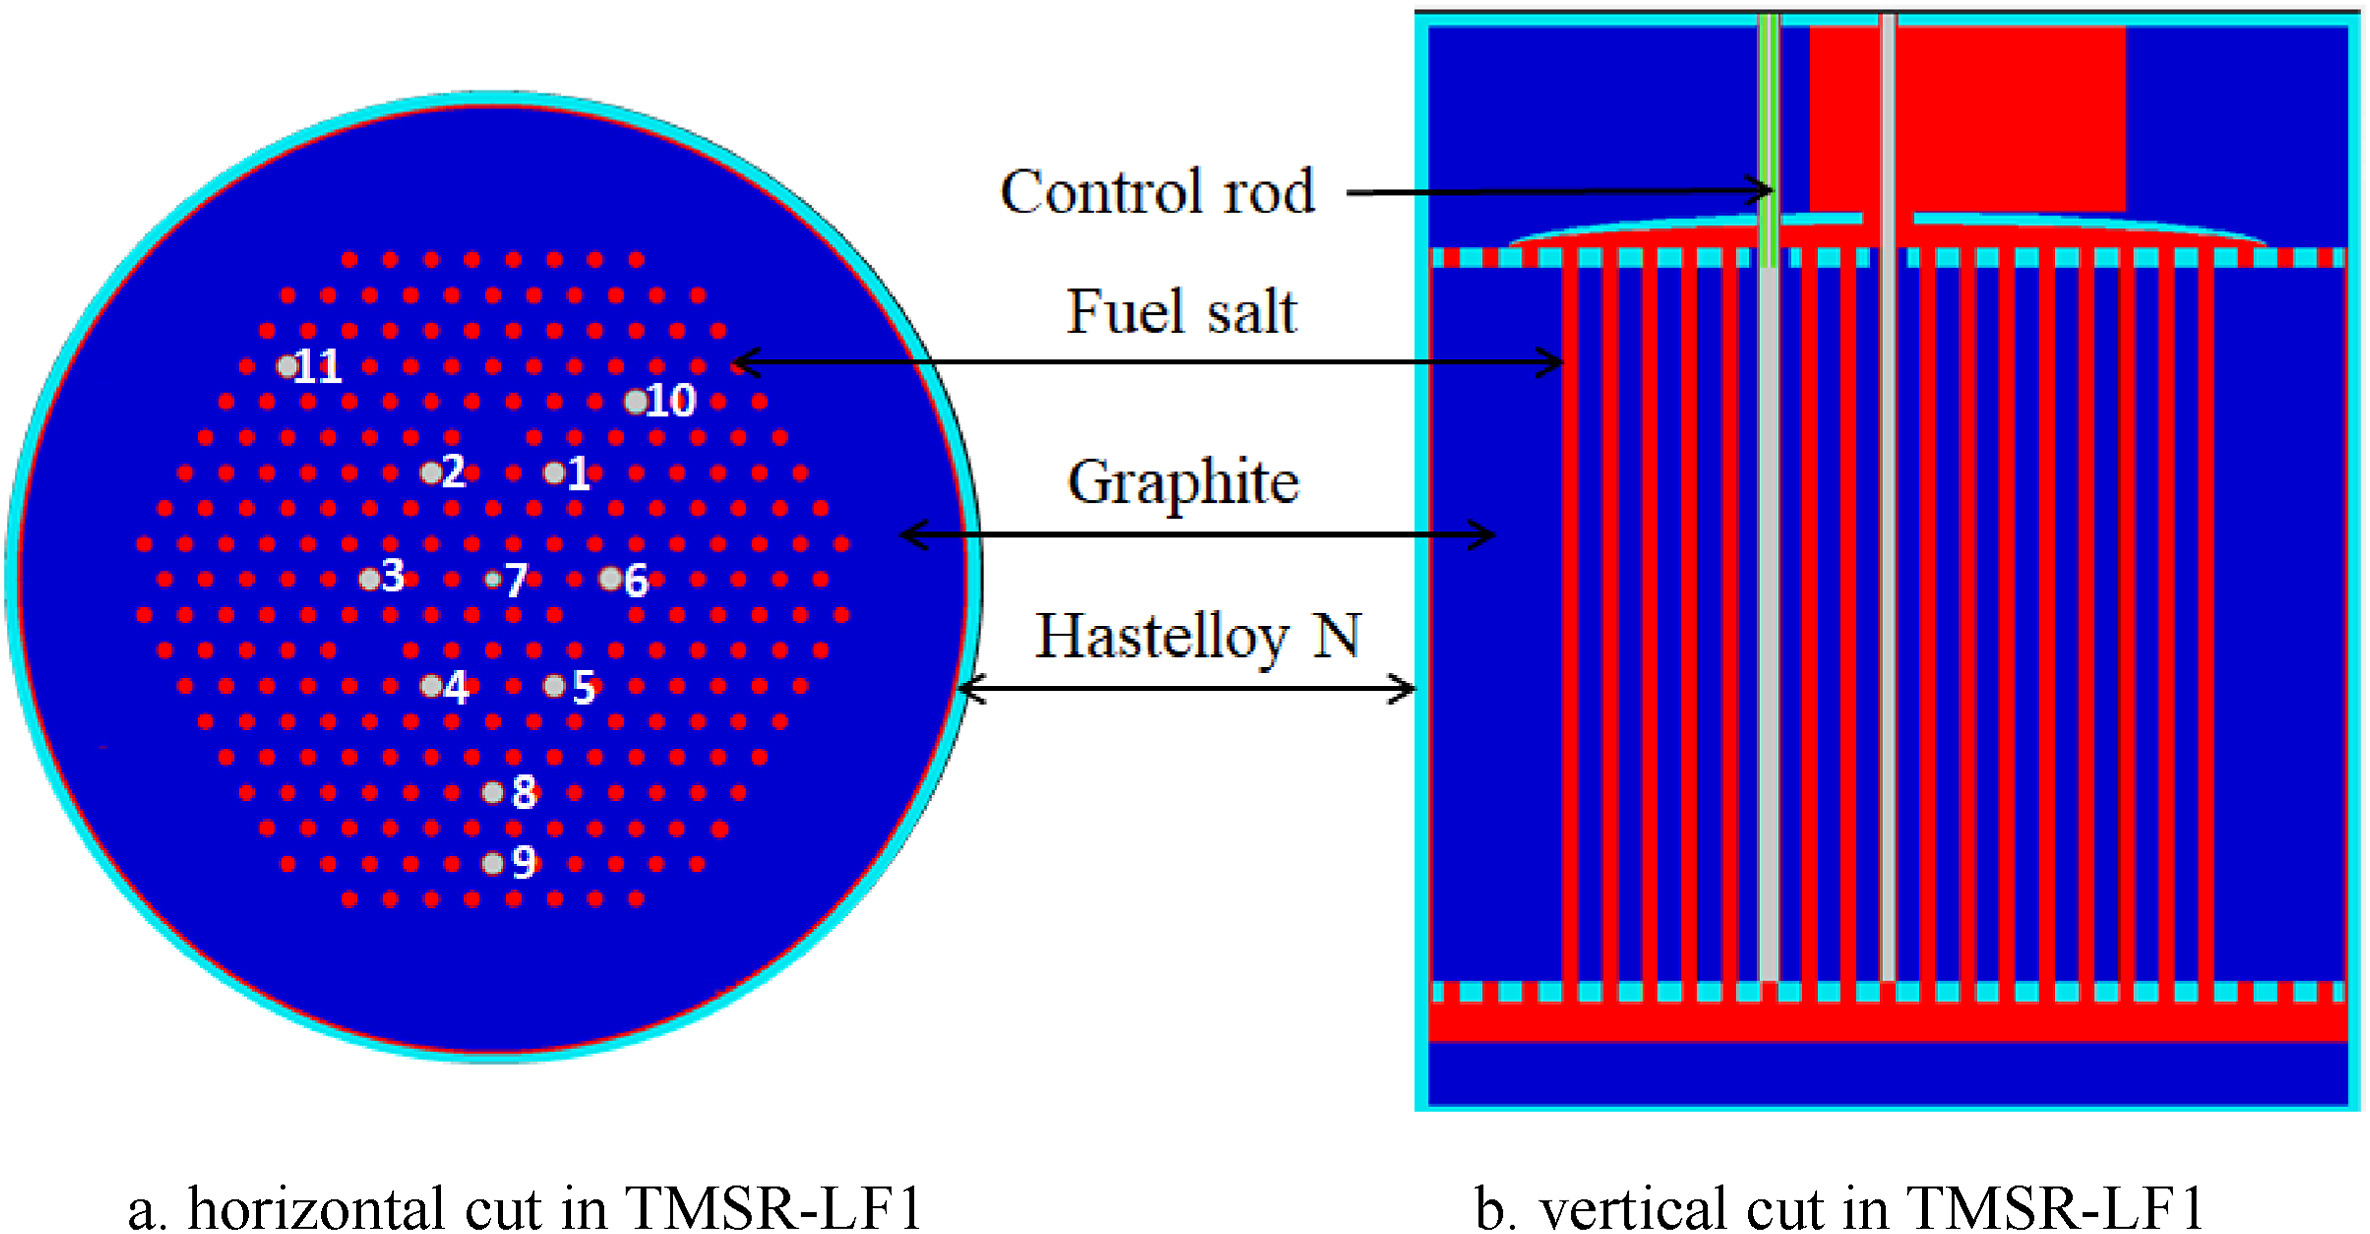
\includegraphics[width=.8\columnwidth]{images/tmsr}
      \caption{\footnotesize Cross-sectional views of the TMSR-LF1
      \cite{liu_sensitivityuncertainty_2020}}
    \end{figure}
    \begin{figure}
      \centering
      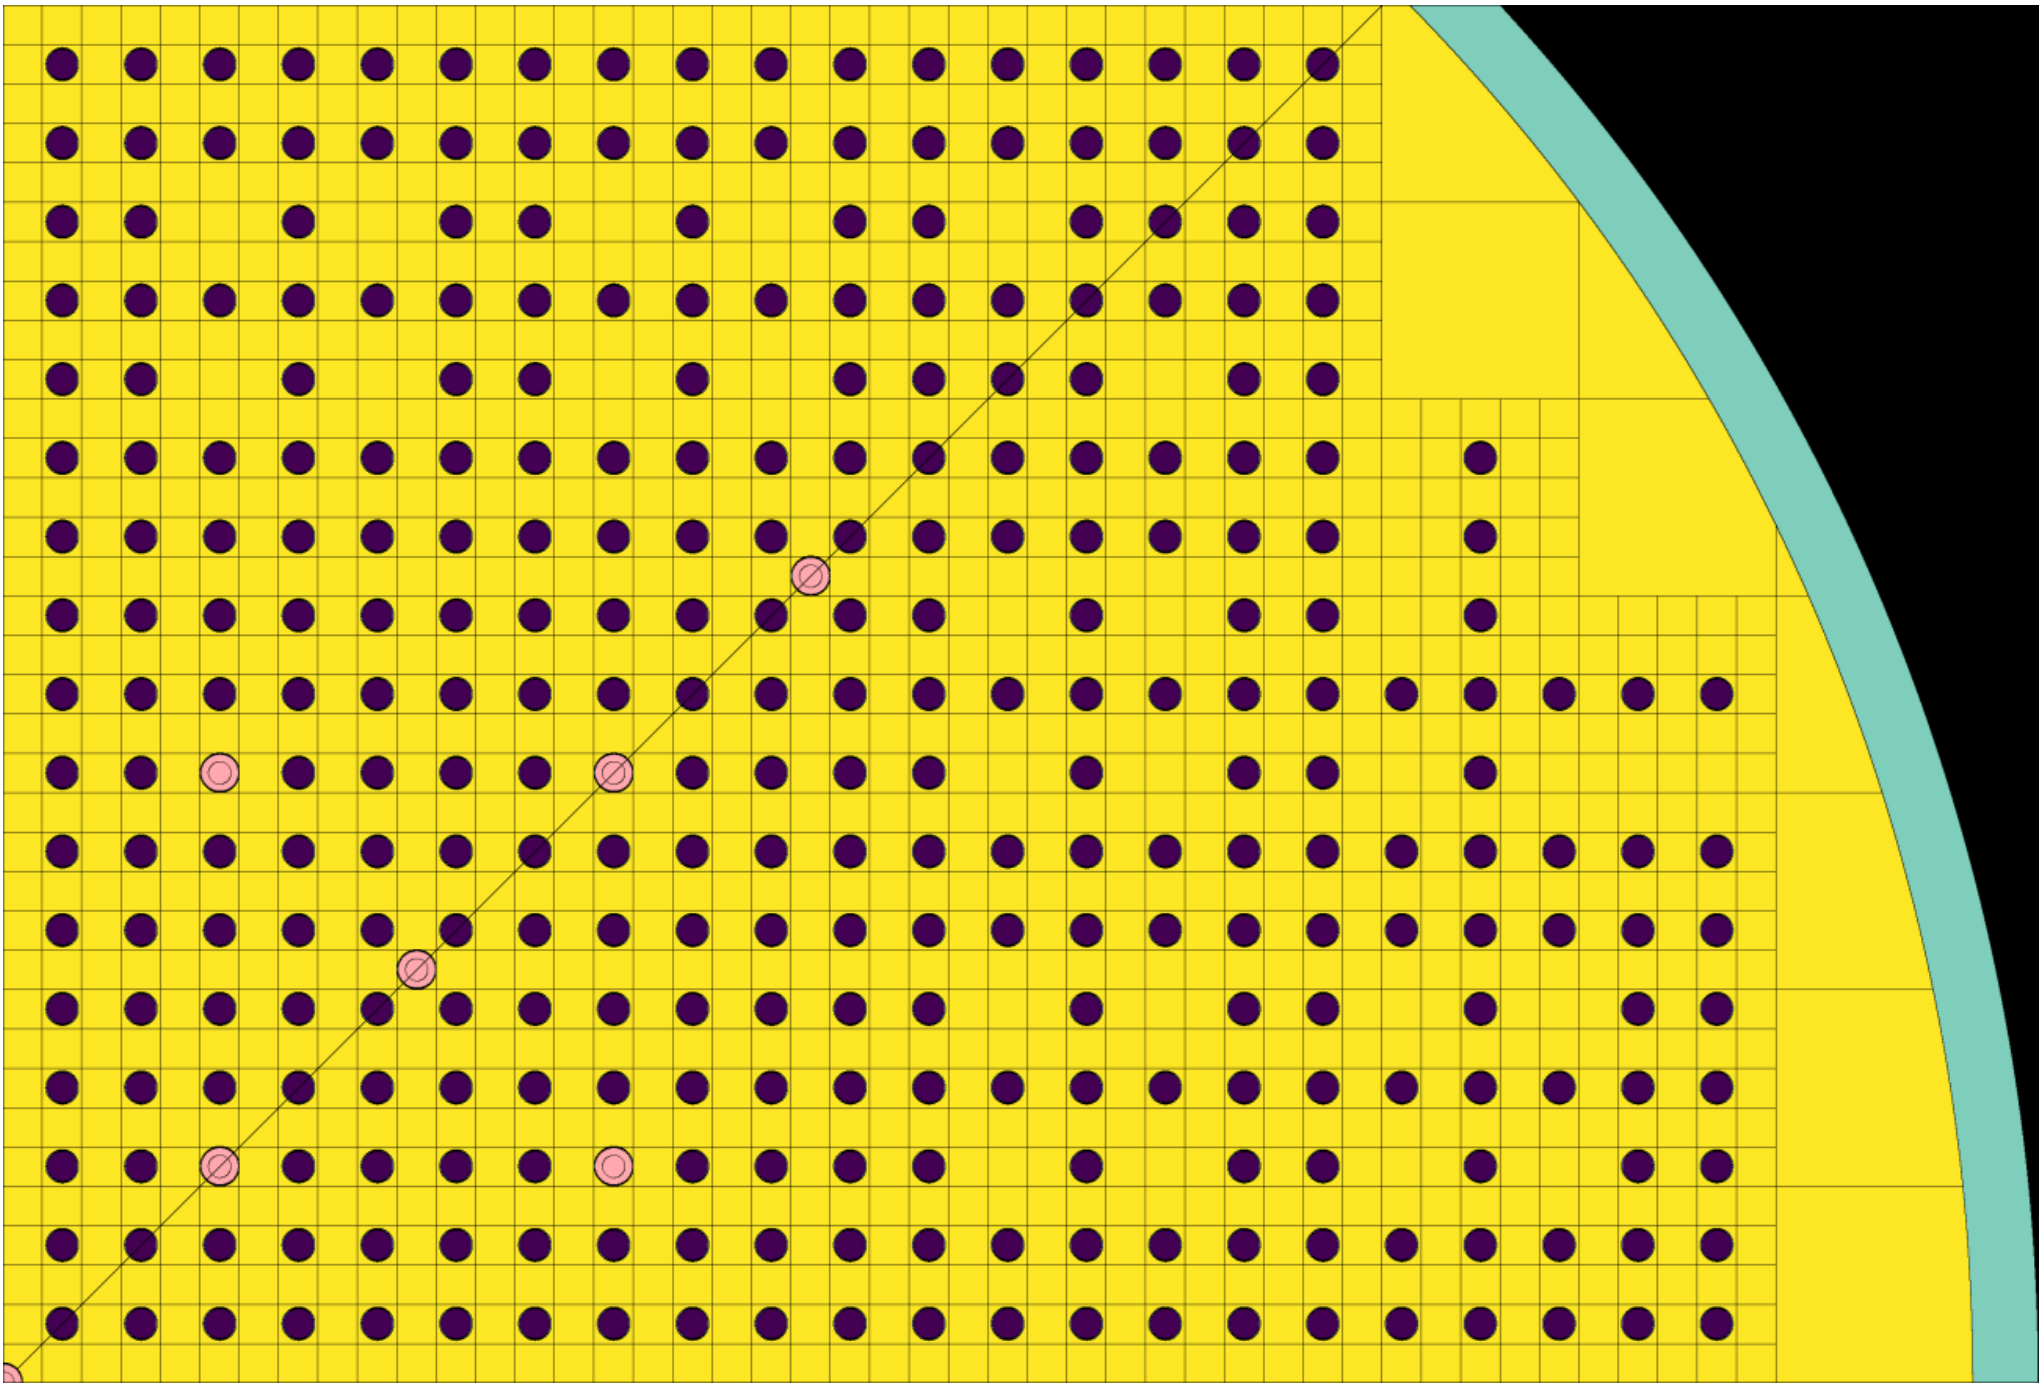
\includegraphics[width=.5\columnwidth]{images/tap-msr-rods}
      \caption{\footnotesize Cross-sectional view of the TAP MSR \cite{lee_neutronics_2020}}
    \end{figure}
    \hfill
  \end{columns}
\end{frame}

\begin{frame}
  \frametitle{Control Rods in MSRs}
  \textbf{Control rods provide a means of controlling the fission rate in nuclear reactors.} 
  \begin{itemize}
    \item Facilitate reactor start-up, shut-down, or load-following operations
    \item Consist of highly neutron-absorbing materials such as boron or gadolinium
  \end{itemize}
  \begin{table}
    \centering
    \footnotesize
    \caption{List of MSR designs which contain control rods.}
    \begin{tabular}{l l}
      \toprule
      Reactor & Spectrum \\
      \midrule
      Molten Salt Reactor Experiment & Thermal \\
      Integral Molten Salt Reactor & Thermal \\
      TMSR-LF1 & Thermal \\
      Liquid Fluoride Thorium Reactor & Thermal \\
      Compact Molten Salt Reactor* & Thermal \\
      Stable Salt Reactor - Wasteburner* & Fast \\
      ThorCon Reactor* & Thermal \\
      \bottomrule
    \end{tabular}
  \end{table}
  Asterisks indicate MSR designs with ``control'' rods labeled as ``shutdown'' rods.
\end{frame}

\begin{frame}
  \frametitle{Control Rod Modeling}
  \textbf{Control rods induce highly anisotropic neutron fluxes and steep flux gradients in their
  vicinity.}
  \pause
  \begin{block}{\textbf{Challenges in Control Rod Modeling in Multiphysics Simulations}}
    \begin{itemize}
      \item \textbf{Neutron diffusion method} performs poorly in regions of low
        scattering-to-absorption ratio and steep neutron flux gradients
      \item \textbf{Neutron transport methods} are computationally costly for time-dependent
        multiphysics simulations (e.g., Monte Carlo, MOC, $S_N$, $P_N$)
    \end{itemize}
  \end{block}
  \pause
  \begin{block}{\textbf{Proposed Work}}
    \textbf{Develop a Hybrid $\bm{S_N}$-Diffusion Method for Control Rod Modeling}
    \begin{itemize}
      \item Applies the discrete ordinates ($S_N$) method around control rods to
        generate corrections for the neutron diffusion equation
      \item Retains the computational efficiency of the neutron diffusion method
    \end{itemize}
  \end{block}
\end{frame}
